\documentclass[13pt]{beamer}
\usepackage{graphicx}
\usepackage[utf8]{inputenc}
\usepackage[skip=2pt,font=scriptsize]{caption}
\usepackage{algorithm}
\usepackage{algorithmic}

% Algorithms
\renewcommand{\algorithmicrequire}{\textbf{Input:}}
\renewcommand{\algorithmicensure}{\textbf{Output:}}
\algsetup{linenosize=\small}

% Captions
\captionsetup{labelformat=empty,labelsep=none}
\DeclareCaptionFormat{myformat}{#3}
\captionsetup[algorithm]{format=myformat}

% References
\usepackage{url}
\bibliographystyle{acm}
\setbeamertemplate{bibliography item}[triangle]

% Formatting
\usetheme{Singapore}
\usecolortheme{whale}

% Title Page
\title{Binomial Heaps}
\author{Devin Delfino}
\institute{Comp 401: Senior Seminar}
\date{3/05/2014}

% Table of Contents
\setbeamertemplate{section in toc}[sections numbered]
\setbeamercolor{alerted text}{fg=blue}
\AtBeginSection[]
{
  \begin{frame}
    \frametitle{Outline}
    \tableofcontents[currentsection]
  \end{frame}
}

\begin{document}
% TITLE ------------------------------------------------
\frame{\titlepage}


% Table of Contents ------------------------------------------------
\begin{frame}
\frametitle{Outline}
\tableofcontents
\end{frame}

\section{Binomial Trees} % ==========================================================================
% BINOMIAL TREES, properties ------------------------------------------------
\begin{frame}
\frametitle{Binomial Trees}
	\begin{itemize}
		\item A \alert{Binomial Tree} is a specific type of tree that includes the following specifications:
          \begin{enumerate}
            \item The \alert{order} or \alert{rank} of the binomial tree is the number of children of the root node.
            \item A Binomial Tree of order $0$ is a single node.
            \item A Binomial Tree of order $k$ has $k$ child nodes, all of which are the roots of binomial trees of orders $k - 1$, $k - 2$, ..., 2, 1, 0 from left to right.
          \end{enumerate}
	\end{itemize}
\end{frame}

% Examples ------------------------------------------------
\begin{frame}
\frametitle{Binomial Trees: Examples}
  \begin{itemize}
    \item If a binomial tree has order \textit{k}, the orders of the \textit{k} child nodes decrease from left to right from $k-1$ to $0$.
  \end{itemize}

  \begin{columns}[T] % the "c" option specifies center vertical alignment
    \begin{column}[T]{3.3cm} % alternative top-align that's better for graphics
      \begin{figure}
        \caption{\textit{k} = 2}
        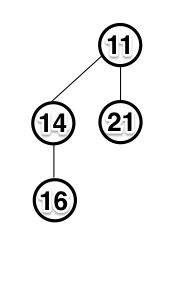
\includegraphics[height=4cm]{./img/order2.png}
      \end{figure}
      \centering
    \end{column}
    \begin{column}[T]{3.3cm} % alternative top-align that's better for graphics
      \begin{figure}
        \caption{\textit{k} = 0}
        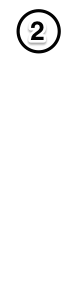
\includegraphics[height=4cm]{./img/order0.png}
      \end{figure}
    \end{column}
    \begin{column}[T]{3.3cm} % alternative top-align that's better for graphics
      \begin{figure}
        \caption{\textit{k} = 3}
        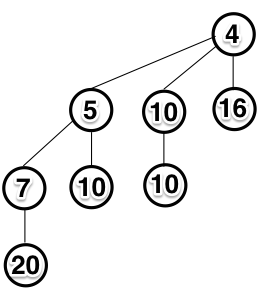
\includegraphics[height=4cm]{./img/order3.png}
      \end{figure}
      \centering
    \end{column}
    \begin{column}[T]{3.3cm} % alternative top-align that's better for graphics
      \begin{figure}
        \caption{\textit{k} = 1}
        
\includegraphics[height=4cm]{./img/order1.png}
      \end{figure}
    \end{column}
  \end{columns}

  % circle subtrees to show the k-1, k-2, ... , 0 sequence
\end{frame}

% BINOMIAL TREES, number of nodes, origin ------------------------------------------------
\begin{frame}
\frametitle{Binomial Trees}
  \begin{itemize}
    \item If a Binomial Tree has an order \textit{k}:
          \begin{enumerate}
            \item The tree has $2^k$ nodes.
            \item The height of the tree is \textit{k}.
            \item There are ${k \choose d}$ nodes at depth \textit{d}.
          \end{enumerate}
    \item ${k \choose d} = \frac{k!}{d! (k - d)!}$ is known as the Binomial Coefficient.
  \end{itemize}

  \begin{columns}[T] % the "c" option specifies center vertical alignment
    \begin{column}[T]{4cm} % alternative top-align that's better for graphics
      \begin{figure}
        \caption{Example: $k = 3$, $d = 2$}
        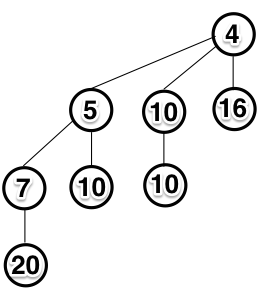
\includegraphics[height=3cm]{./img/order3.png}
      \end{figure}
      \centering
    \end{column}
    \begin{column}[T]{7cm} % alternative top-align that's better for graphics
      $$
        {k \choose d} = {3 \choose 2} = \frac{3!}{2! (3 - 2)!} = \frac{6}{2 * 1} = \frac{6}{2} = 3
      $$
    \end{column}
  \end{columns}
\end{frame}

\section{Binomial Heaps} % ==========================================================================
% BINOMIAL HEAP ------------------------------------------------
\begin{frame}
\frametitle{Binomial Heaps}
  \begin{itemize}
    \item A \alert{Binomial Heap} is a collection of binomial trees that satisfy the following two binomial heap properties:
      \begin{enumerate}
        \item The key of any node is greater than or equal to the key of its parent (minimum-heap property).
        \item There cannot be two binomial trees of the same order.
      \end{enumerate}
    % \item Binomial heaps are used to implement priority queues.
  \end{itemize}
\end{frame}

% BINOMIAL HEAP, property 1 ------------------------------------------------
\begin{frame}
\frametitle{Binomial Heap: Property \#1 (minimum-heap)}
  \begin{itemize}
    \item The first property (minimum-heap) ensures that the root is the smallest key in each binomial tree.
    \item The smallest key of the entire heap is one of the roots.
  \end{itemize}

  \begin{columns}[T] % the "c" option specifies center vertical alignment
    \begin{column}[T]{6.5cm} % alternative top-align that's better for graphics
      \begin{figure}
        \caption{Min-Heap Property $\checkmark$}
        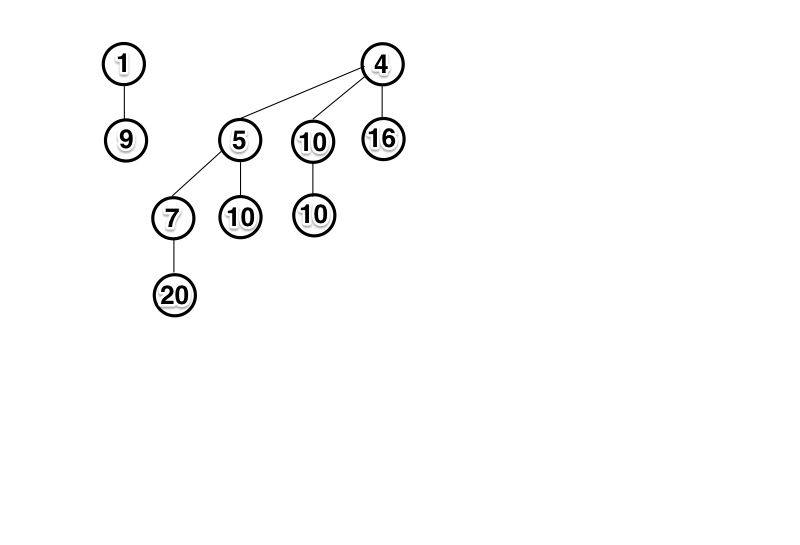
\includegraphics[height=7cm]{./img/minheap1.png}
      \end{figure}
      \centering
    \end{column}
    \begin{column}[T]{6.5cm} % alternative top-align that's better for graphics
      \begin{figure}
        \caption{Min-Heap Property $\times$}
        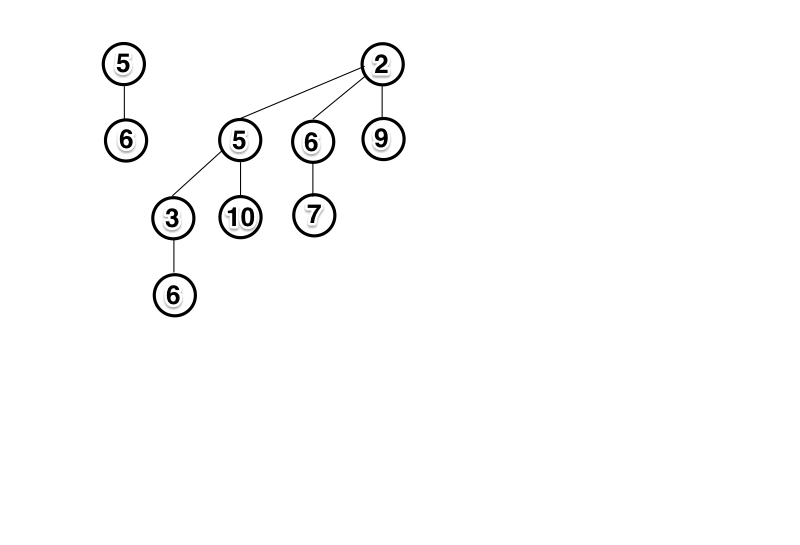
\includegraphics[height=7cm]{./img/minheap2.png}
      \end{figure}
    \end{column}
  \end{columns}
\end{frame}

% BINOMIAL HEAP, property 2 ------------------------------------------------
\begin{frame}
\frametitle{Binomial Heap: Property \#2}
  \begin{itemize}
    \item The order of each binomial tree must be unique.
  \end{itemize}

  \begin{columns}[T] % the "c" option specifies center vertical alignment
    \begin{column}[T]{4.3cm} % alternative top-align that's better for graphics
      \begin{figure}
        \caption{Property \#2 $\times$}
        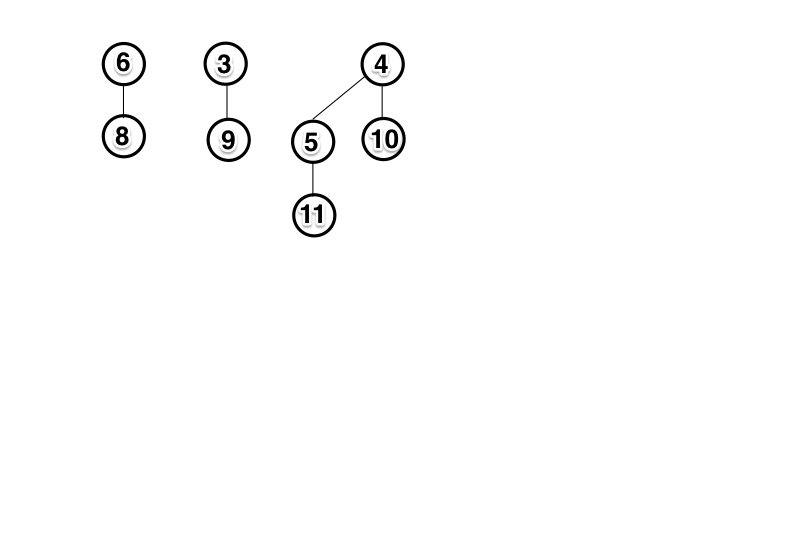
\includegraphics[height=5cm]{./img/struct4.png}
      \end{figure}
      \centering
    \end{column}
    \begin{column}[T]{4.3cm} % alternative top-align that's better for graphics
      \begin{figure}
        \caption{Property \#2 $\checkmark$}
        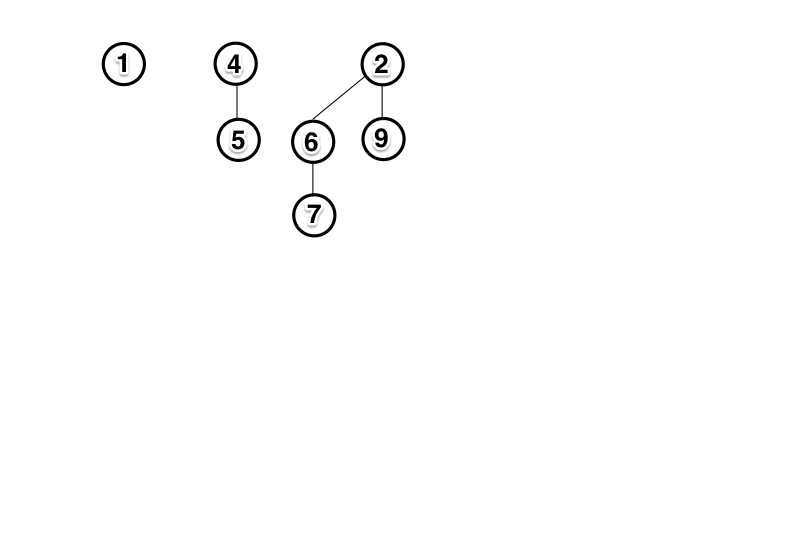
\includegraphics[height=5cm]{./img/struct2.png}
      \end{figure}
    \end{column}
    \begin{column}[T]{4.3cm} % alternative top-align that's better for graphics
      \begin{figure}
        \caption{Property \#2 $\times$}
        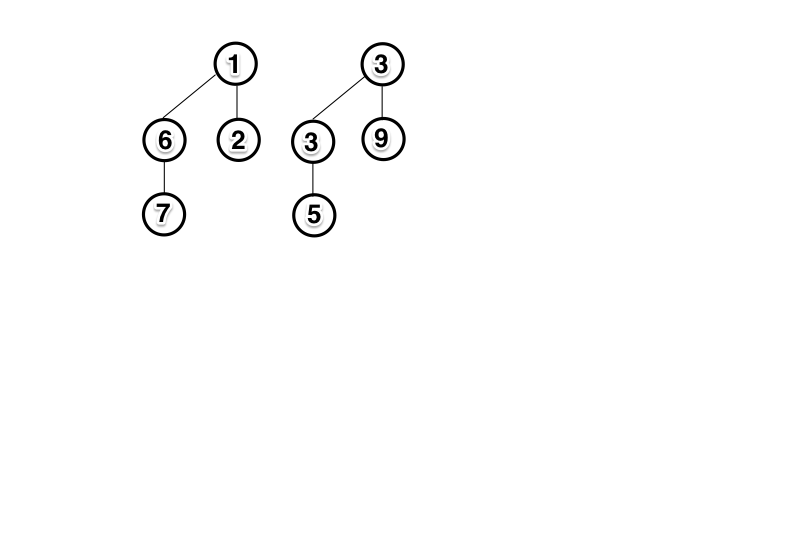
\includegraphics[height=5cm]{./img/struct1.png}
      \end{figure}
    \end{column}
  \end{columns}

\end{frame}

% BINOMIAL HEAP ------------------------------------------------
\begin{frame}
\frametitle{Binomial Heap: Property \#2, Cont.}
  \begin{itemize}
    \item The second property ensures that if a binomial heap has \textit{n} nodes, then it will have at most $\lfloor \textit{log n} \rfloor + 1$ binomial trees.
    \item The total number of nodes can also be thought of as a binary string, where each binomial tree represents a bit.
  \end{itemize}

  \begin{figure}
    % \caption{$11 = 2^0 + 2^1 + 2^2 + 2^3 \Rightarrow 1011$}
    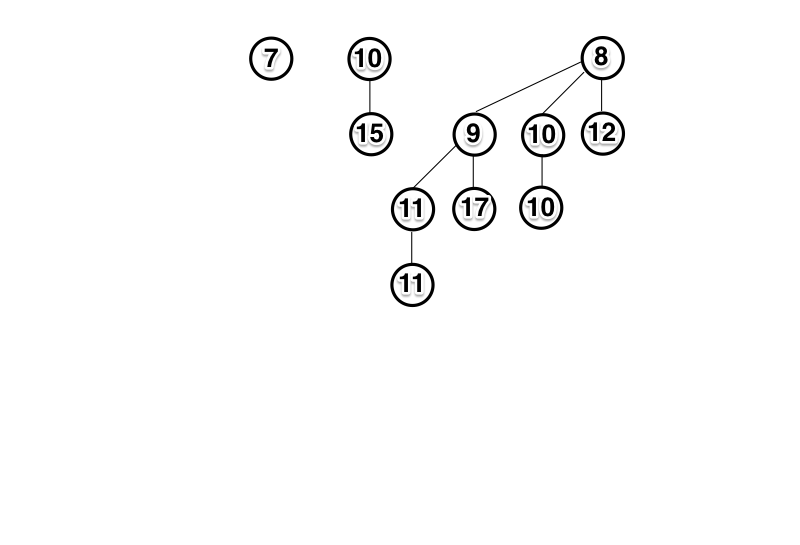
\includegraphics[height=7.5cm]{./img/bheap.png}
  \end{figure}

    % explain the log n (surrounded by powers of 2)
% explain both bullet points and show hidden caption
\end{frame}

\section{Implementation Structure} % ==========================================================================
% BINOMIAL HEAP ------------------------------------------------
\begin{frame}
\frametitle{Implementation Structure}
  
\begin{figure}
    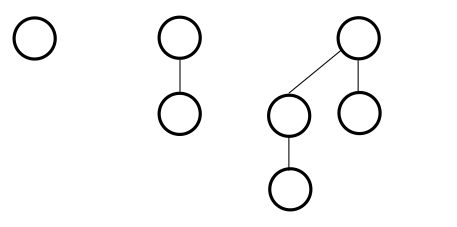
\includegraphics[height=6cm]{./img/structimp.png}
\end{figure}

\end{frame}

\section{Standard Functions} % ==========================================================================
% Merge ------------------------------------------------
% during slide 1, draw merged output
\begin{frame}
\frametitle{Standard Functions: Merge}
  \begin{itemize}
    \item Two $k$ ordered binomial trees are merged into one $k + 1$ ordered binomial tree.
  \end{itemize}

  \begin{columns}[T] % the "c" option specifies center vertical alignment
    \begin{column}[T]{6cm} % alternative top-align that's better for graphics
        \begin{algorithm}[H]
        \small
        \caption{Merge}
        \begin{algorithmic}
          \REQUIRE Node* root\_A, Node* root\_B

          \IF{root\_A.key $\leq$ root\_B.key}
            \STATE root\_B.right\_sibling $\leftarrow$ root\_A.child
            \STATE root\_A.child $\leftarrow$ root\_B
            \STATE root\_B.parent $\leftarrow$ root\_A
            \RETURN root\_A
          \ELSE
            \STATE root\_A.right\_sibling $\leftarrow$ root\_B.child
            \STATE root\_B.child $\leftarrow$ root\_A
            \STATE root\_A.parent $\leftarrow$ root\_B
            \RETURN root\_B
          \ENDIF
        \end{algorithmic}
        \end{algorithm}
    \end{column}
    \begin{column}[T]{5.5cm} % alternative top-align that's better for graphics
      \begin{figure}
        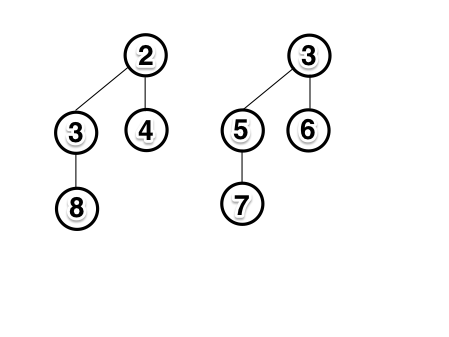
\includegraphics[height=5cm]{./img/premerge.png}
      \end{figure}
    \end{column}
  \end{columns}

\end{frame}

\begin{frame}
\frametitle{Standard Functions: Merge}
  \begin{itemize}
    \item Two $k$ ordered binomial trees are merged into one $k + 1$ ordered binomial tree.
  \end{itemize}

  \begin{columns}[T] % the "c" option specifies center vertical alignment
    \begin{column}[T]{6cm} % alternative top-align that's better for graphics
        \begin{algorithm}[H]
        \small
        \caption{Merge}
        \begin{algorithmic}
          \REQUIRE Node* root\_A, Node* root\_B

          \IF{root\_A.key $\leq$ root\_B.key}
            \STATE root\_B.right\_sibling $\leftarrow$ root\_A.child
            \STATE root\_A.child $\leftarrow$ root\_B
            \STATE root\_B.parent $\leftarrow$ root\_A
            \RETURN root\_A
          \ELSE
            \STATE root\_A.right\_sibling $\leftarrow$ root\_B.child
            \STATE root\_B.child $\leftarrow$ root\_A
            \STATE root\_A.parent $\leftarrow$ root\_B
            \RETURN root\_B
          \ENDIF
        \end{algorithmic}
        \end{algorithm}
    \end{column}
    \begin{column}[T]{5.5cm} % alternative top-align that's better for graphics
      \begin{figure}
        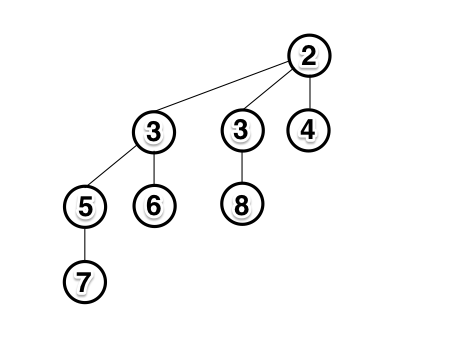
\includegraphics[height=5cm]{./img/postmerge.png}
      \end{figure}
    \end{column}
  \end{columns}

\end{frame}

% Join ------------------------------------------------
\begin{frame}
\frametitle{Standard Functions: Join}
  \begin{itemize}
    \item
  \end{itemize}
\end{frame}

% Insert ------------------------------------------------
\begin{frame}
\frametitle{Standard Functions: Insert}
  \begin{itemize}
    \item
  \end{itemize}
\end{frame}

% DeleteMinimum ------------------------------------------------
\begin{frame}
\frametitle{Standard Functions: DeleteMinimum}
  \begin{itemize}
    \item
  \end{itemize}

  \begin{columns}[T] % the "c" option specifies center vertical alignment
    \begin{column}[T]{6cm} % alternative top-align that's better for graphics
        \begin{algorithm}[H]
        \small
        \caption{BinomialHeap : DeleteMinimum}
        \begin{algorithmic}
          \REQUIRE None

          \STATE Node* deleted\_node $\leftarrow$ this\_heap.FindMinimum()
          \STATE BinomialHeap temp\_heap $\leftarrow$ new BinomialHeap()
          \FOR{each \textit{child} in delete\_node}
              \STATE temp\_heap.insert(child)
          \ENDFOR
          \STATE this\_heap.join(temp\_heap)
        \end{algorithmic}
        \end{algorithm}
    \end{column}
    \begin{column}[T]{5.5cm} % alternative top-align that's better for graphics
      \begin{figure}
        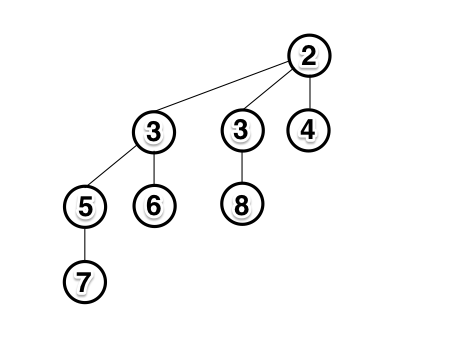
\includegraphics[height=5cm]{./img/postmerge.png}
      \end{figure}
    \end{column}
  \end{columns}
\end{frame}

% DecreaseKey ------------------------------------------------------------------------------------------
\begin{frame}
\frametitle{Standard Functions: DecreaseKey}
  \begin{itemize}
    \item Decreases the key of a given node in the Binomial Heap
  \end{itemize}

  \begin{columns}[T] % the "c" option specifies center vertical alignment
    \begin{column}[T]{6cm} % alternative top-align that's better for graphics
        \begin{algorithm}[H]
        \small
        \caption{BinomialHeap : DecreaseKey}
        \begin{algorithmic}
          \REQUIRE Node* node, int new\_key

          \STATE decrease\_node.key $\leftarrow$ new\_key
          \STATE Node* temp $\leftarrow$ decrease\_node
          \WHILE{temp.parent $\neq$ NULL}
              \IF{temp.key $<$ temp.parent.key}
                \STATE swap(temp.key, temp.parent.key)
              \ELSE
                \STATE break
              \ENDIF
              \STATE temp $\leftarrow$ temp.parent
          \ENDWHILE
        \end{algorithmic}
        \end{algorithm}
    \end{column}
    \begin{column}[T]{7cm} % alternative top-align that's better for graphics
      \begin{figure}
        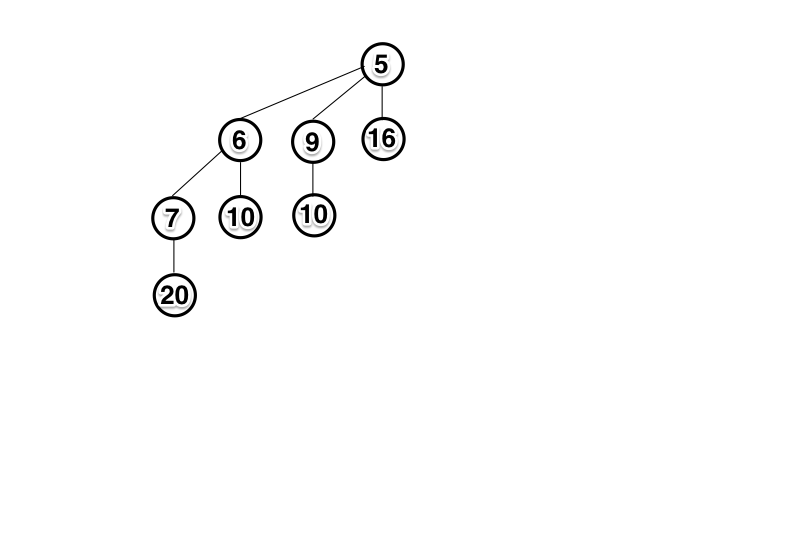
\includegraphics[height=8cm]{./img/decreasekeyA.png}
      \end{figure}
    \end{column}
  \end{columns}

\end{frame}

\begin{frame}
\frametitle{Standard Functions: DecreaseKey}
  \begin{itemize}
    \item Decreases the key of a given node in the Binomial Heap
  \end{itemize}

  \begin{columns}[T] % the "c" option specifies center vertical alignment
    \begin{column}[T]{6cm} % alternative top-align that's better for graphics
        \begin{algorithm}[H]
        \small
        \caption{BinomialHeap : DecreaseKey}
        \begin{algorithmic}
          \REQUIRE Node* node, int new\_key

          \STATE decrease\_node.key $\leftarrow$ new\_key
          \STATE Node* temp $\leftarrow$ decrease\_node
          \WHILE{temp.parent $\neq$ NULL}
              \IF{temp.key $<$ temp.parent.key}
                \STATE swap(temp.key, temp.parent.key)
              \ELSE
                \STATE break
              \ENDIF
              \STATE temp $\leftarrow$ temp.parent
          \ENDWHILE
        \end{algorithmic}
        \end{algorithm}
    \end{column}
    \begin{column}[T]{7.5cm} % alternative top-align that's better for graphics
      \begin{figure}
        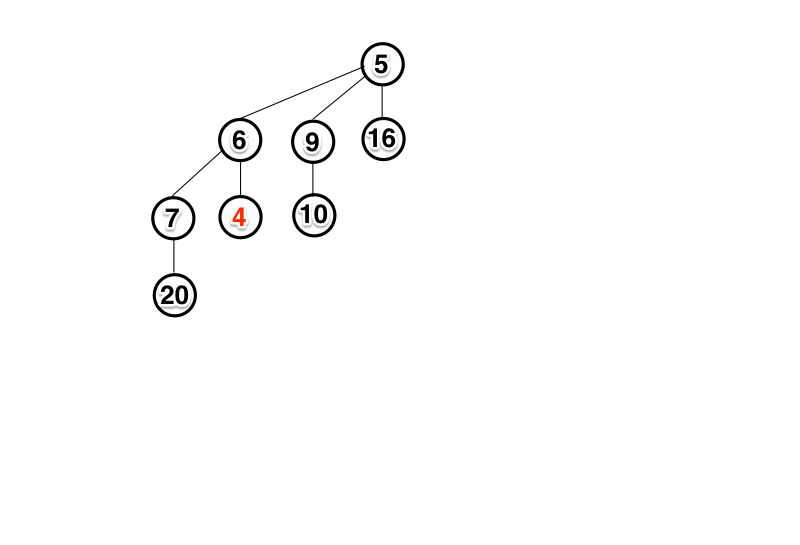
\includegraphics[height=8cm]{./img/decreasekeyB.png}
      \end{figure}
    \end{column}
  \end{columns}

\end{frame}

\begin{frame}
\frametitle{Standard Functions: DecreaseKey}
  \begin{itemize}
    \item Decreases the key of a given node in the Binomial Heap
  \end{itemize}

  \begin{columns}[T] % the "c" option specifies center vertical alignment
    \begin{column}[T]{6cm} % alternative top-align that's better for graphics
        \begin{algorithm}[H]
        \small
        \caption{BinomialHeap : DecreaseKey}
        \begin{algorithmic}
          \REQUIRE Node* node, int new\_key

          \STATE decrease\_node.key $\leftarrow$ new\_key
          \STATE Node* temp $\leftarrow$ decrease\_node
          \WHILE{temp.parent $\neq$ NULL}
              \IF{temp.key $<$ temp.parent.key}
                \STATE swap(temp.key, temp.parent.key)
              \ELSE
                \STATE break
              \ENDIF
              \STATE temp $\leftarrow$ temp.parent
          \ENDWHILE
        \end{algorithmic}
        \end{algorithm}
    \end{column}
    \begin{column}[T]{7.5cm} % alternative top-align that's better for graphics
      \begin{figure}
        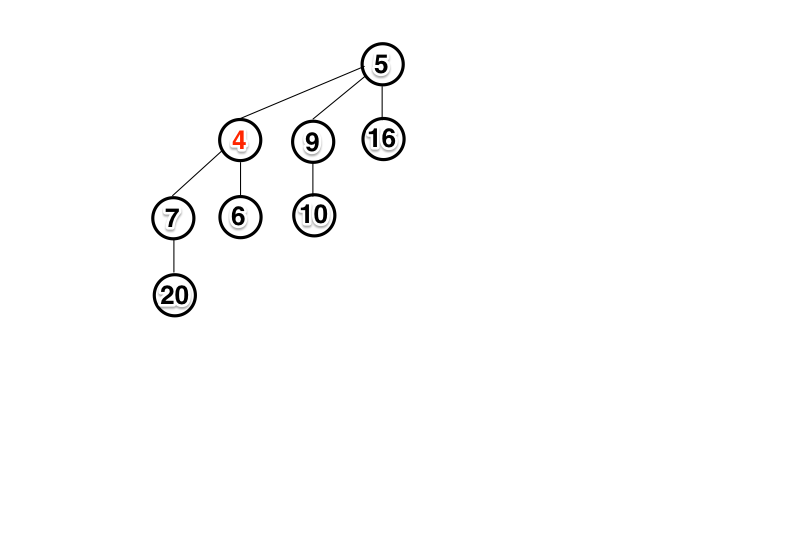
\includegraphics[height=8cm]{./img/decreasekeyC.png}
      \end{figure}
    \end{column}
  \end{columns}

\end{frame}

\begin{frame}
\frametitle{Standard Functions: DecreaseKey}
  \begin{itemize}
    \item Decreases the key of a given node in the Binomial Heap
  \end{itemize}

  \begin{columns}[T] % the "c" option specifies center vertical alignment
    \begin{column}[T]{6cm} % alternative top-align that's better for graphics
        \begin{algorithm}[H]
        \small
        \caption{BinomialHeap : DecreaseKey}
        \begin{algorithmic}
          \REQUIRE Node* node, int new\_key

          \STATE decrease\_node.key $\leftarrow$ new\_key
          \STATE Node* temp $\leftarrow$ decrease\_node
          \WHILE{temp.parent $\neq$ NULL}
              \IF{temp.key $<$ temp.parent.key}
                \STATE swap(temp.key, temp.parent.key)
              \ELSE
                \STATE break
              \ENDIF
              \STATE temp $\leftarrow$ temp.parent
          \ENDWHILE
        \end{algorithmic}
        \end{algorithm}
    \end{column}
    \begin{column}[T]{7.5cm} % alternative top-align that's better for graphics
      \begin{figure}
        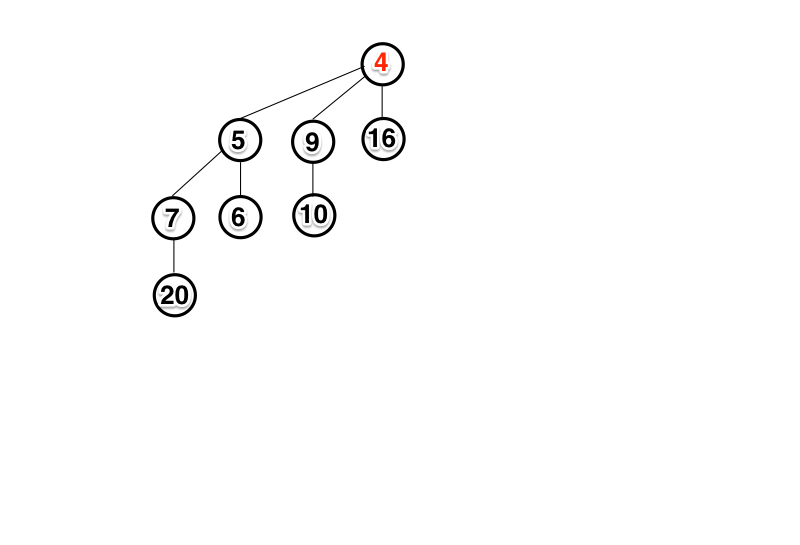
\includegraphics[height=8cm]{./img/decreasekeyD.png}
      \end{figure}
    \end{column}
  \end{columns}

\end{frame}

% Delete -----------------------------------------------------------------------------------------------
\begin{frame}
\frametitle{Standard Functions: Delete}
  \begin{itemize}
    \item Deletes a given node from the Binomial Heap
  \end{itemize}

  \begin{columns}[T] % the "c" option specifies center vertical alignment
    \begin{column}[T]{9cm} % alternative top-align that's better for graphics
        \begin{algorithm}[H]
        \small
        \caption{BinomialHeap : Delete}
        \begin{algorithmic}
          \REQUIRE Node* delete\_node

          \STATE BinomialHeap.DecreaseKey(delete\_node, $-9999$)
          \STATE BinomialHeap.DeleteMinimum()
        \end{algorithmic}
        \end{algorithm}
    \end{column}
  \end{columns}

  \begin{figure}
    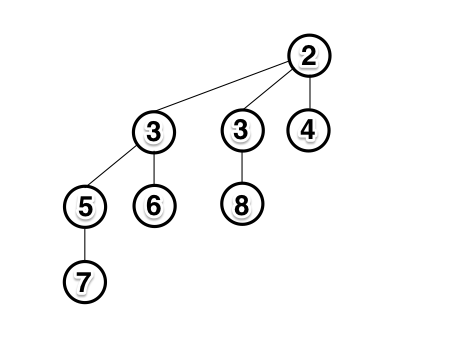
\includegraphics[height=5cm]{./img/postmerge.png}
  \end{figure}

\end{frame}

\section{Uses of Binomial Heaps} % ==========================================================================
% BINOMIAL HEAP ------------------------------------------------
\begin{frame}
\frametitle{Uses of Binomial Heaps}
  \begin{itemize}
    \item A \alert{Binomial Heap} is a collection of binomial trees that satisfy the following two binomial heap properties:
      \begin{enumerate}
        \item The key of any node is greater than or equal to the key of its parent (minimum-heap property).
        \item There cannot be two binomial trees of the same order.
      \end{enumerate}
    % \item Binomial heaps are used to implement priority queues.
  \end{itemize}
\end{frame}

% References ------------------------------------------------
 \begin{frame}
  \frametitle{References}
  \nocite{*} 
  \bibliography{workscited}
\end{frame}

\end{document}